\section{Модели}

\subsection{YOLOv5}

YOLO (You Only Look Once) -- архитектура одностадийной нейронной сети для обнаружения объектов в режиме реального времени, созданная в 2015 году Джозефом Редмоном в университете Вашингтона, главными преимуществами которой являются скорость работы и легковесность.

В 2016 году была выпущена YOLOv2 (YOLO9000) \cite{5-2}, ставшая улучшением оригинальной модели, включив в нее пакетную нормализацию, якорные рамки и кластеры размерности, а также позволившая детектировать объекты из 9000 категорий. YOLOv3 \cite{5-3} была выпущена в 2018 году и усовершенствовала эффективность модели за счет использования более результативной базовой части и добавления пирамид признаков.

В 2020 году была выпущена модель YOLOv4 \cite{5-4}, в которой появился ряд нововведений, таких как использование мозаичной аугментации данных и новая функция потерь. В этом же году команда Ultralytics выпустила реализованную на PyTorch YOLOv5, продемонстрировав резкий скачок в производительности модели.

\begin{figure}[ht]
    \centering
    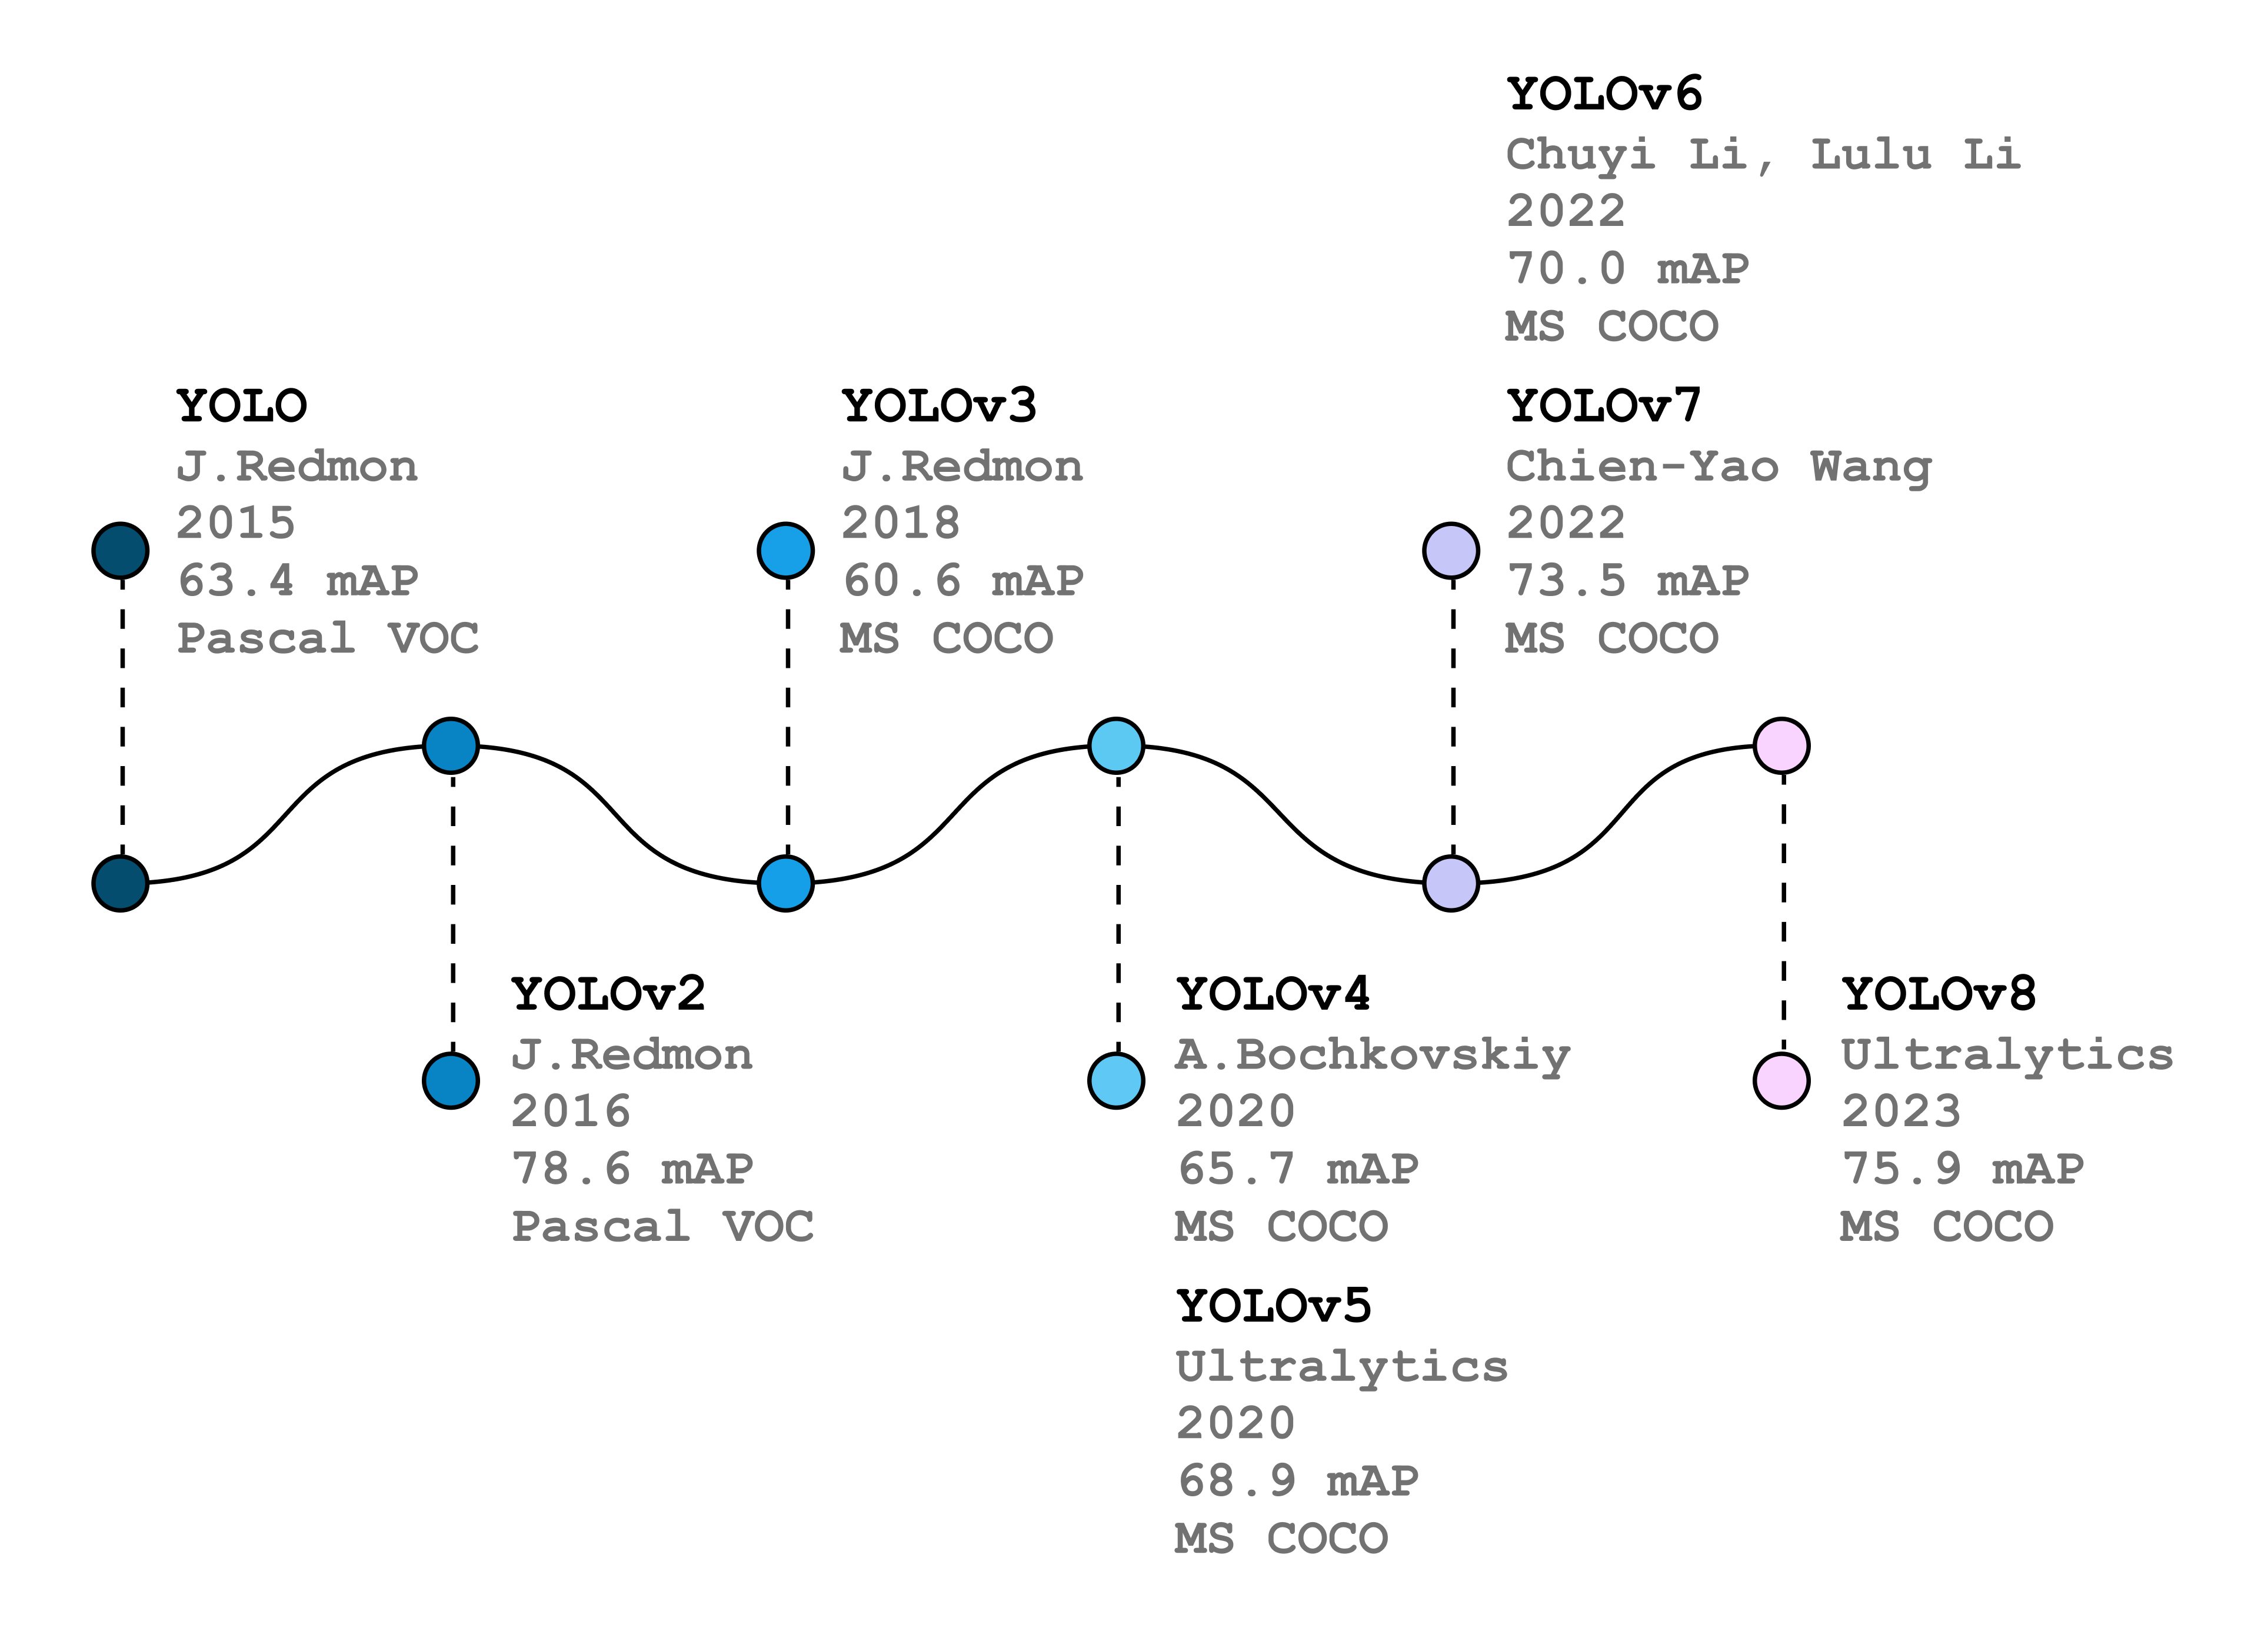
\includegraphics[width=0.85\textwidth]{5-1}
    \caption{История YOLO}
    \label{img:5-1}
\end{figure}

Архитектура используемой одностадийной модели состоит из 3 компонент: Backbone, Neck и Dense Prediction, как показано на Рис. \ref{img:5-1}. Backbone, являющаяся предварительно обученной сетью и используемая для извлечения признаков изображений, способствует уменьшению их разрешения и увеличению пространства признаков. Компонента Neck, используемая для извлечения пирамид признаков, создана для объединения информации с отдельных слоев предыдущих блоков и позволяет модели обобщенно работать с объектами разных размеров и масштабов. Блок Head используется для выполнения операций на заключительном этапе, добавляя якорные рамки к картам признаков и реализуя вывод конечных результатов: классов объектов, оценок точности предсказаний и ограничивающих рамок.

\vspace{0.5cm}

\begin{figure}[ht]
    \centering
    \includegraphics[width=0.85\textwidth]{5-2}
    \caption{Структура одностадийного детектора}
    \label{img:5-2}
\end{figure}

YOLOv5 \cite{5-4} применяет в качестве компоненты Backbone CSP-Darknet53, сверточную нейронную сеть Darknet53, использованную в качестве основы для YOLOv3, к которой применена Cross Stage Partial (CSP). В качестве Neck использованы Spatial Pyramid Pooling (SPP), преимущество которого в значительном увеличении рецептивного поля и выделении наиболее значимых контекстных признаков без снижения скорости работы сети, и Path Aggregation Network (PANet), модифицированная путем добавления BottleNeckCSP в ее архитектуру. Head состоит из трех слоев свертки, которые предсказывают расположение ограничивающих рамок, оценки точности и классы объектов. Схема данной структуры представлена на Рис. \ref{img:5-2}.

\begin{figure}[ht]
    \centering
    \includegraphics[width=0.85\textwidth]{5-3}
    \caption{Схема структуры модели YOLOv5}
    \label{img:5-3}
\end{figure}

По сравнению с предыдущими моделями были представлены новые формулы для вычисления координат ограничивающих рамок, решающие проблему ранних версий с неправильным детектированием объектов в углах и по краям изображений:

\begin{equation}
    b_x = (2 \cdot \sigma(t_x) - 0.5) + c_x
\end{equation}

\begin{equation}
    b_y = (2 \cdot \sigma(t_y) - 0.5) + c_y
\end{equation}

\begin{equation}
    b_w = p_w \cdot (2 \cdot e^{t_w})^2
\end{equation}

\begin{equation}
    b_h = p_h \cdot (2 \cdot e^{t_h})^2
\end{equation}

\vspace{0.5cm}

Концепция работы YOLO, особенность которой состоит в просмотре всего изображения целиком за один раз, представляет собой деление изображения на области размером $S \times S$ одинакового размера, каждая из которых отвечает за обнаружение центра объекта внутри нее и предсказание фиксированного количества ограничивающих рамок с определенным уровнем достоверности нахождения объекта внутри нее. Далее при помощи IoU происходит выбор наиболее подходящих из полученных рамок, а последующее удаление лишних из оставшихся -- через немаксимальное подавление (NMS).
